Introducing the Kubernetes specific vocabulary used through the cluster manager
will make the following discussions of auto-scaling easier. In addition to
describing each component of Kubernetes in general, Figure
\ref{fig:kubernetes-visualization-no-autoscaler} presents an overview of the
interaction between the different building blocks which compose Kubernetes.
Figure \ref{fig:kubernetes-visualization-no-autoscaler} also gives a sense of
the lifecycle of an external request from an external client
to a service running on Kubernetes.
Importantly, this visualization shows just one service. Multiple different
services can be run on a Kubernetes cluster, each with their own service,
replication controller, and pods.

\begin{figure}[!h]
  \centerline{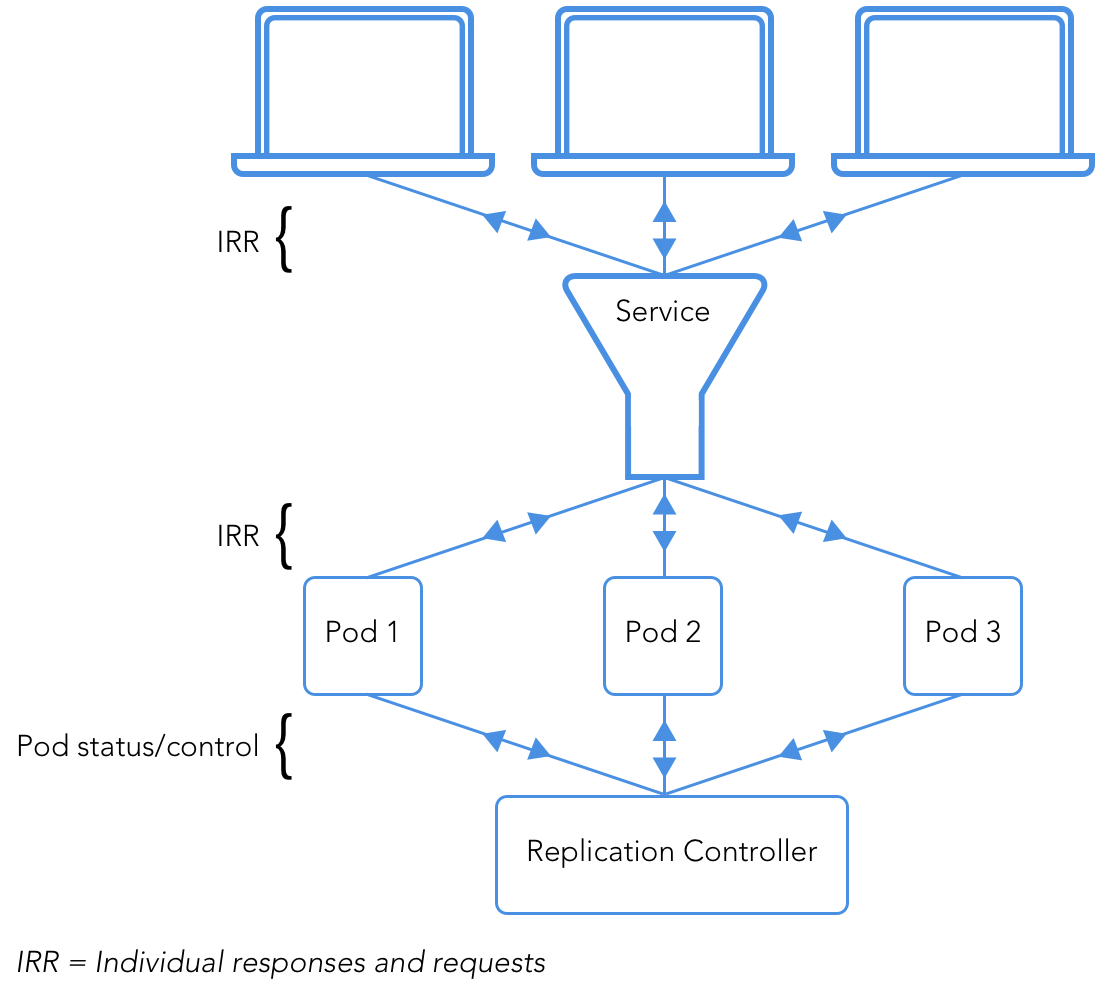
\includegraphics[scale=.25]{kubernetes-visualization-no-autoscaler.png}}
  \caption{A visualization showing a client making requests to a
  sample service running on Kubernetes.}
  \label{fig:kubernetes-visualization-no-autoscaler}
\end{figure}

\subsection{Pods}

The \textit{pod} is the smallest deployable unit that Kubernetes can create and
manage. A pod can contain one or more
containerized applications, and one or more pods can run on a physical host
machine. Multiple applications should run on the same pod
if these applications need to be run in the same
physical machine; otherwise, the applications should be in separate pods.
Containerized applications within a pod can see each others' processes,
access the same IP network, and share the same host name. Like well-designed
containers within the microservices model, well-designed pods should be
focused, stateless, and concurrent, as Kubernetes assumes that pods can be deleted,
created, and replicated at will. The user can either submit a
single pod to Kubernetes to schedule and run on a node in the cluster, or
multiple replica pods
can be created by a replication controller \cite{k8s-pods}.


\subsection{Replication Controllers}

As mentioned in the previous section, pods can be created by a replication
controller. A replication controller is responsible for ensuring that a given
number of replica pods are constantly running. It does this by restarting any
deleted or terminated pods. Though the replication controller performs a
seemingly simple task, it is useful for scaling the number of pods and
performing a rolling update of the pod \cite{k8s-replication-controllers}.

Additionally, auto-scaling is closely associated with replication controllers, as
auto-scalers are attached to replication controllers for pods. In short, the
auto-scaler tells the replication controller how many pods should exist, and the
replication controller ensures that number of pods exist and are operating
successfully. This relationship will be discussed in considerably more detail later when
examining the architecture and implementation of auto-scaling in Kubernetes in
Section \ref{architecture-autoscaling-in-kubernetes}
\cite{k8s-horizontal-pod-autoscaler-proposal}.


\subsection{Services}

The final main architectural building block of Kubernetes is the \textit{service}.
Services are necessary because pods are ephemeral. As a pod may be deleted or
replaced at any time, it is important that no entity is trying to communicate
with a specific pod, because that pod may disappear. Instead, entities wishing to
communicate with a pod always establish contact with a consistent service.
A service presents a single, long-running access point
for multiple replica pods, as the service receives
external requests to the pods, and load-balances
these requests across the replicas.\footnote{The replication of
these pods is handled by a replication controller.} This endpoint is used within
a Kubernetes cluster as pods wish to communicate with each other and it can also
be exposed outside of the cluster. Again, the concept of a service is
particularly important to auto-scaling, as when the replication
controller creates pod replicas, the services ensures work is balanced across
them. This load-balancing, and the knowledge of the new replicas on which to
share the load, is entirely automated \cite{k8s-services}.

